\subsubsection{Cadre Général}

Ce module entre en action après stimulation de la phase d'analyse qui lui fournit, par l'intermédiaire de la mémoire, l'environnement courant et un ensemble de formes reconnues. Le \og moteur de choix \fg{} se sert alors de la probabilité d'apparition des annotations associées aux formes reconnues afin d'annoter l'environnement courant.

\subsubsection{Application aux jeux de plateau}

Dans le cadre des jeux de plateau, le moteur de choix obtient un ensemble de plateaux, chacun associé à un ensemble de formes reconnues. Chaque plateau correspond au plateau résultant d'un coup possible. On peut donc dire que ce moteur doit choisir entre les différents \og futurs possibles \fg{}.

Afin d'évaluer la probabilité de gain d'un plateau, celui-ci fera la moyenne des probabilités de gain des différentes formes reconnues sur ce plateau. Il choisi finalement l'environnement qui maximise la probabilité de gain.

\begin{figure}[H] 
  \begin{center}
		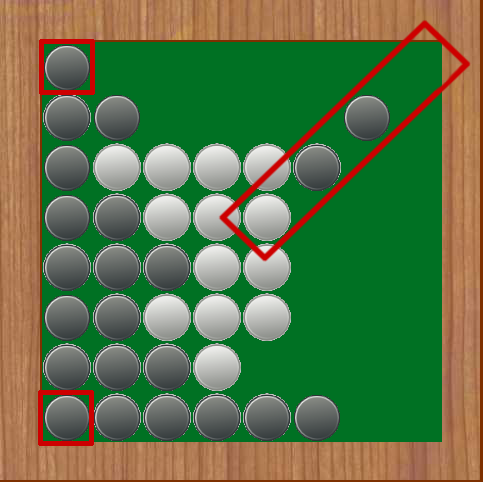
\includegraphics[width=0.3\textwidth]{files/raisonneur/moteur_de_choix} 
	\end{center}
\caption{Représentation graphique de l'environnement.} 
\label{img_env}
\end{figure}
